\begin{frame}{Templates}{Introduction}
	A good LaTeX software package will contain at least some standard templates
	for different document types such as articles, beamers, and books, a great one will also
	let you create your own template. \vspace{1em}

	Templates can be very useful when there are certain
	documents types you need to create often such as class notes, homework assignments, and lab reports.
\end{frame}

\begin{frame}[fragile]{Templates}{Elements in a template}
    \footnotesize
    Custom commands can be made on the fly by using the \texttt{newcommand}.
    Similarly we can use \texttt{newenvironment}.

    
\includegraphics[width=0.8\textwidth]{template1.png}
    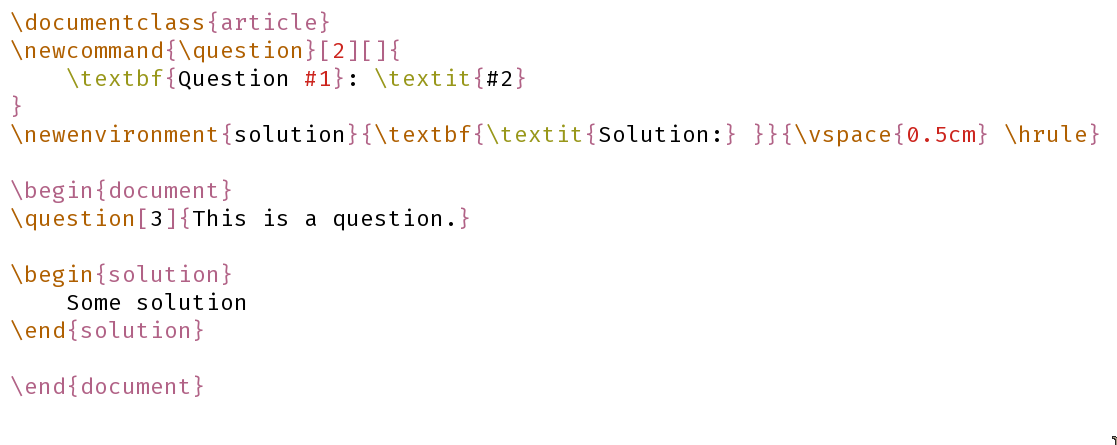
\includegraphics[width=0.8\textwidth]{template1_code.png}
\end{frame}


\begin{frame}[fragile]{Templates}{Counters}
    \footnotesize
    There is a counter, automatically counts up everytime it is called.

    \begin{columns}
        \begin{column}{0.3\textwidth}
            
\includegraphics[width=\textwidth]{template2.png}
        \end{column}
        \begin{column}{0.7\textwidth}
            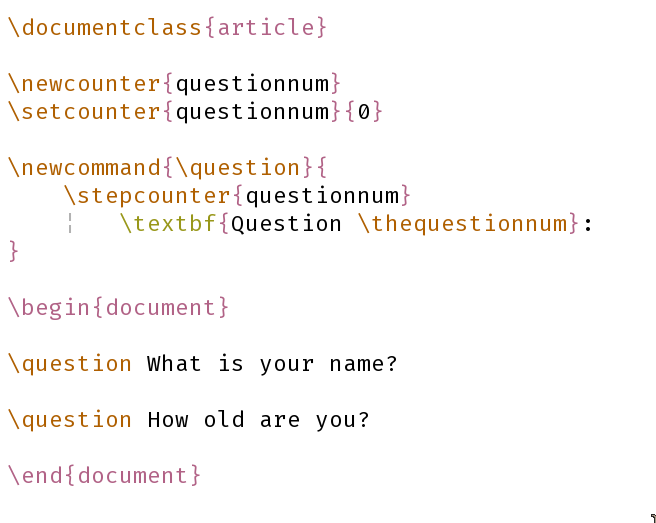
\includegraphics[width=\textwidth]{template2_code.png}
        \end{column}
    \end{columns}
\end{frame}



\begin{frame}{Templates}{Task-6}
    Try to solve Task-6.
\end{frame}
